\documentclass[tikz]{standalone}
\usepackage{amsmath}
\usepackage{xcolor}
\usetikzlibrary{calc}

\begin{document}
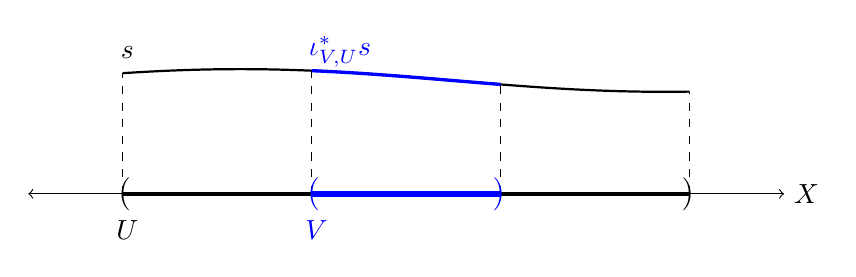
\begin{tikzpicture}[scale=1.2]

  % Axis
  \draw[<->] (0,0) -- (8,0) node[right] {$X$};

  % Parameters for intervals
  \coordinate (Uleft)  at (1,0);
  \coordinate (Uright) at (7,0);
  \coordinate (Vleft)  at (3,0);
  \coordinate (Vright) at (5,0);

  % Draw interval U: black, thicker but not as thick as blue V
  \draw[line width=1.2pt, black] (Uleft) -- (Uright);


  % Label U under the line
  \node[below=6pt] at (1.05, 0) {$U$};

  % Draw interval V: thick blue line
  \draw[blue, line width=2pt] (Vleft) -- (Vright);

 
  % Label V under the line (near)
  \node[below=6pt, blue] at (3.05, 0) {$V$};

  % Define gentle functions:
  % s(x) = 0.12*sin(0.7*x) + 1.2   (over U)
  % t(x) = 0.12*sin(1.2*x) + 1.9   (over V, slightly higher)
  %
  % (We will use these exact expressions below inside plot)

  % Full function s over U
  \draw[domain=1:7,smooth,variable=\x,thick]
    plot ({\x},{0.12*sin(0.7*\x r) + 1.2});
  \node at (1.05,1.5) {$s$};

  % Highlight restriction: portion of s over V as thick blue
  \draw[domain=3:5,smooth,variable=\x,blue,very thick]
    plot ({\x},{0.12*sin(0.7*\x r) + 1.2});
  \node[blue] at (3.3, 1.5) {$\iota_{V,U}^* s$};

  % Dashed vertical edges from U endpoints up to s
  \draw[dashed] plot coordinates {(1,0) (1,{0.12*sin(0.7*1 r) + 1.2})};
  \draw[dashed] plot coordinates {(7,0) (7,{0.12*sin(0.7*7 r) + 1.2})};

  % Dashed vertical edges from V endpoints up to s
  \draw[dashed] plot coordinates {(3,0) (3,{0.12*sin(0.7*3 r) + 1.2})};
  \draw[dashed] plot coordinates {(5,0) (5,{0.12*sin(0.7*5 r) + 1.2})};

   % Parentheses for V in blue
  \node[blue] at (3.02, 0)  {\large (};
  \node[blue] at (4.98, 0) {\large )};

  % Parentheses for U (literal characters positioned at endpoints)
  \node at (1.02, 0)  {\large (};
  \node at (6.98, 0) {\large )};


\end{tikzpicture}
\end{document}
